\part{Streszczenie}
Niniejszy dokument zawiera wyniki pomiaru czasu, którego potrzebował mój komputer na zapełnienie zaimplementowanych przeze mnie struktur danych opartych na typach tablicowych: stos, kolejka oraz lista zestawami danych o długościach od 1 do 1e7 elementów. Zawiera także dokumentację kodu, który pojawił się w projekcie od poprzedniego sprawozdania.

\part{Sprawozdanie}
Obliczenia wykonano na 64-bitowym procesorze AMD Athlon X2. Wszystkie implementacje zostały badane pod kątem najgorszego scenariusza. Wykresy przedstawiają porównania zależnośći czasu wykonywania operacji od długości ciągu danych dla różnych implementacji poszczególnych struktur. Porównywane implementacje to: \newline
- kontenery z biblioteki standardowej, \newline
- implementacja z użyciem list jednokierunkowych, \newline
- z użyciem tablic, gdzie pojemność tablicy jest zwiększana o jeden element,\newline
- z użyciem tablic, gdzie pojemność tablicy zwiększana jest dwukrotnie.
\vspace{0.5cm}
\newpage
\centerline{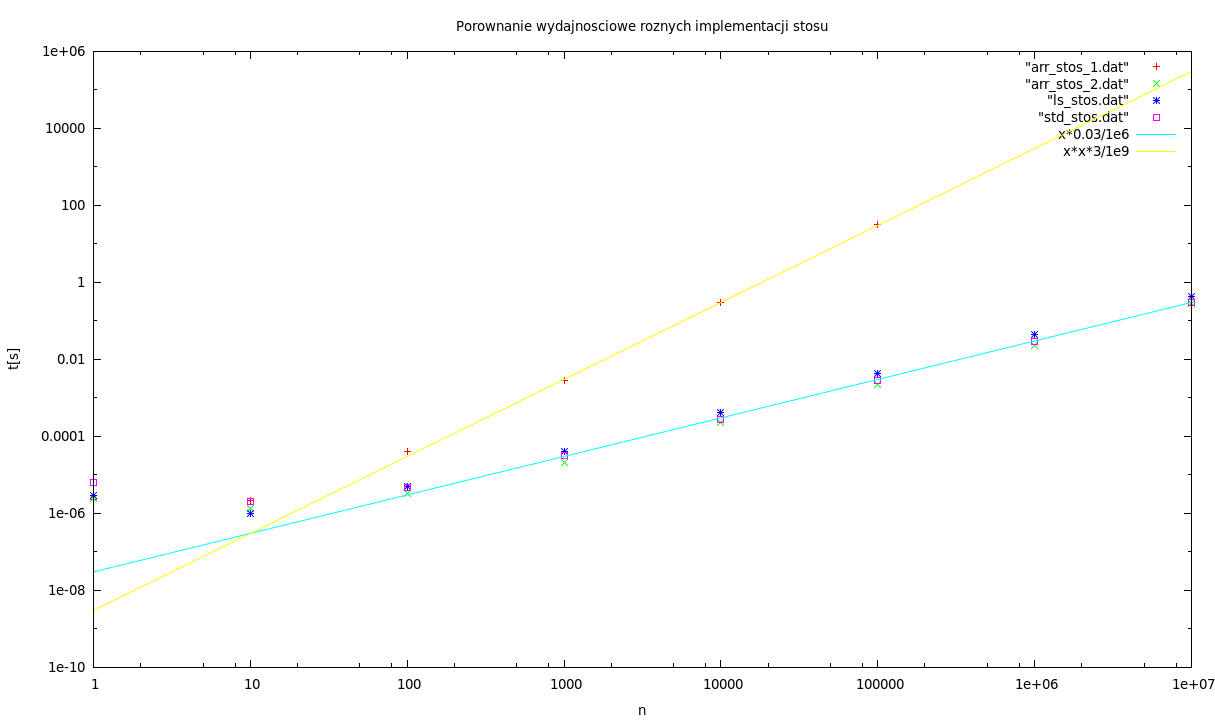
\includegraphics[width=\textwidth,height=\textheight, keepaspectratio]{stos.png}}
Wykres 1. Porównanie różnych implementacji stosu.
\newline
% ### KOMENTARZ DO 1. WYKRESU
Zależność czasu wykonywania operacji od ilości danych wrzucanych na szczyt stosu dla wszystkich implementacji z wyjątkiem tablicowej-zwiększanej-o-1 dobrze aproksymuje linia prosta po czym można przypuszczać, że złożoność tej operacji jest \begin{math}O(n)\end{math}. Dla stosu z biblioteki standardowej i zaimplementowanego za pomocą listy jest to trafny wniosek, gdyż ich złożoność jest faktycznie liniowa. Inaczej jest w przypadku stosu tablicowego-powiększanego-dwukrotnie, bowiem w trakcie powiększania go co jakiś czas następuje przepisanie całej jego zawartośći do innego miejsca w pamięci, co oczywiście jest operacją liniową. Jednak w związku z tym, że wraz ze zwiększaniem się ilości danych na stosie częstotliwość wystąpienia operacji przenoszenia maleje, wzrasta wydajność czasowa kosztem wydajności pamięciowej. Jak widać na wykresie, prosta bardzo dobrze aproksymuje stopień złożoności dla tej implementacji.

W przypadku stosu tablicowego-powiększanego-o-1 za każdym razem, gdy wyczerpiemy zapas pojemności kontenera, następuje realokacja całej jego zawartości do nowego miejsca z zapasem mogącym zmieścić jeden element - ten zapas wyczerpuje się w momencie, w którym wrzucimy na stos kolejny element. W konsekwencji wrzucenie na stos \begin{math}n\end{math} danych kosztuje nas \begin{math}n\end{math}-krotne \begin{math}n\end{math} przepisań całego stosu, co razem daje \begin{math}n^{2}\end{math} operacji, zatem złożoność obliczeniowa tego przedsięwzięcia wynosi \begin{math}O(n^{2})\end{math}.Gdyby wykres był w skali liniowej, linia aproksymująca współrzędne uzyskane z badań nad tą implementacją byłaby ramieniem paraboli.
\newpage
\centerline{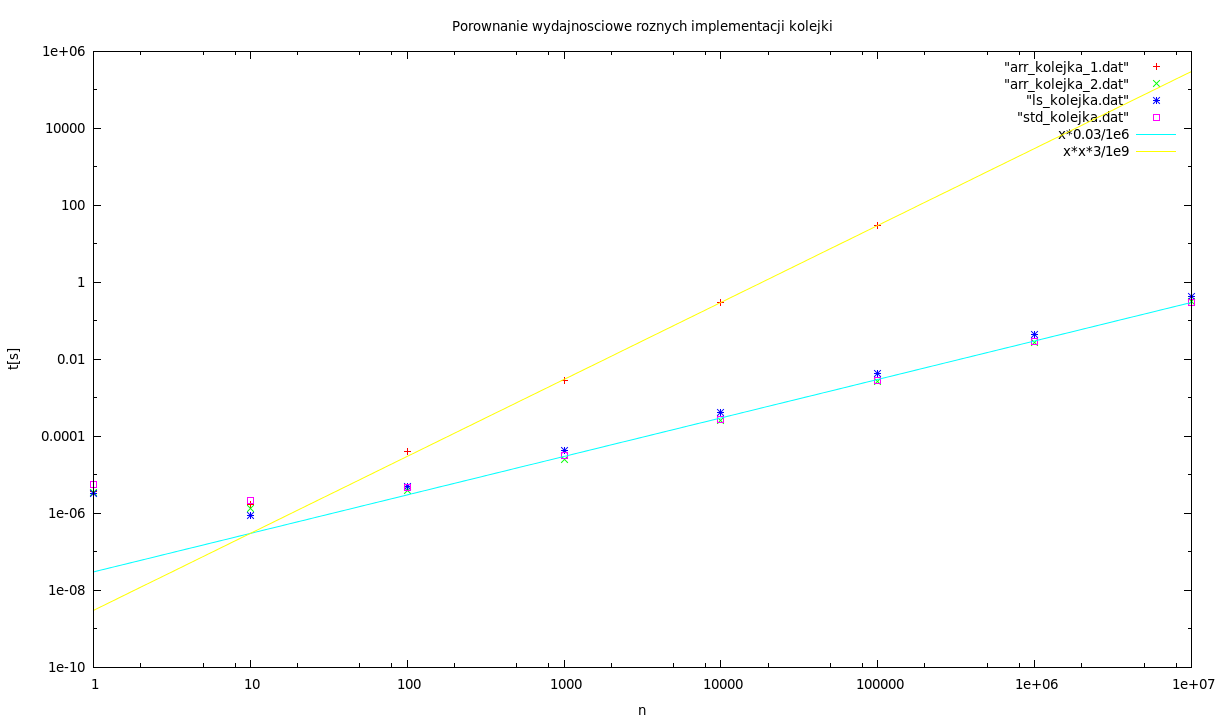
\includegraphics[width=\textwidth,height=\textheight, keepaspectratio]{kolejka.png}}
Wykres 2. Porównanie różnych implementacji kolejki.
\newline
% ### KOMENTARZ DO 2. WYKRESU

Sytuacja jest identyczna jak w przypadku stosu - ze względu na sposób implementacji wyniki są prawie identyczne. Różnice w tych strukturach byłyby widoczne, gdyby badano zdejmowanie z nich elementów.
\newpage
\centerline{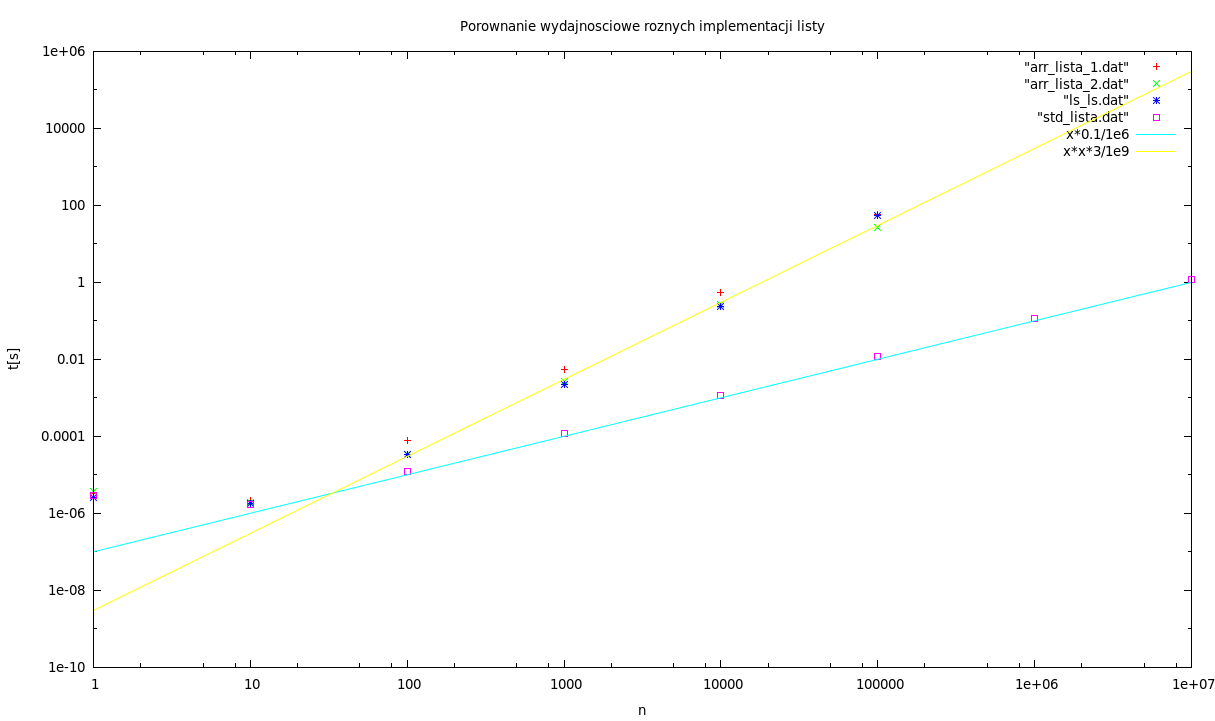
\includegraphics[width=\textwidth,height=\textheight, keepaspectratio]{lista.png}}
Wykres 3. Porównanie różnych implmentacji listy.
\newline
% ### KOMENTARZ DO 3. WYKRESU
Jedyną implementacją, w której umieszczanie elementów ma złożoność liniową jest lista z biblioteki standardowej. Jest to spodowane tym, że std::list wykorszytane do porównania jest listą dwukierunkową i nie jest wymagane każdorazowe przesuwanie jej zawartości podczas dodawania do niej elementu.

Złożoność obliczeniowa wszystkich moich implementacji jest \begin{math}O(n^{2})\end{math}, ponieważ napisana przez mnie lista jednokierunkowa została zaprojektowana w taki sposób, że dodawanie na jej początek nowego elementu (co jest najgorszym scenariuszem pod względem złożoności) wymaga operacji na każdym elemencie istniejącym w liście - jest to przesuwanie wskaźnika pomocniczego z końca na sam początek listy lub podnoszenie każdego elementu o jedno miejsce bliżej końca. Mamy więc dla \begin{math}n\end{math}-elemenotwego zbioru danych \begin{math}n\end{math}-krotne\begin{math} n\end{math} przesunięć wektora służące wpięciu nowego elementu listy na jej początek lub, w przypadku implementacji tablicowej, \begin{math}n\end{math}-krotne \begin{math}n\end{math} podniesień elementów bliżej końca by zrobić miejsce na nowy element w indeksie zerowym. 
\newpage
